\documentclass[a4paper,11pt]{article}

%\usepackage[latin1]{inputenc}
%\usepackage[utf-8]{inputenc}
\usepackage[english]{babel}

\usepackage{amssymb}
\usepackage{amsmath}

\usepackage[bottom=1.38in, top=1.5in, left=1.5in, right=1.5in]{geometry}

\usepackage{graphicx}
\usepackage{subfigure}
\usepackage{wrapfig}

\usepackage{fontspec}
\usepackage{xunicode}
\usepackage{xltxtra}

\usepackage{setspace}

%\usepackage[T1]{fontenc}
%\usepackage[sc]{mathpazo}

\defaultfontfeatures{Mapping=tex-text, Scale=MatchLowercase}
\setmainfont{Gentium}
% \setromanfont{Gentium}
% \setsansfont{Lucida Grande}
% \setmonofont{Menlo}


% \def\gauthor{Esben Skaarup}
% \def\gauthordetails{, npl306, sben@sben.dk}
% \def\gtitle{Proactive Computer Security \\ Week 1 - Web Security}
% \def\gshorttitle{PCS - Web Security}
% \def\gdate{\today}

%Define commands
\newcommand{\systemname}{Pre-tested Integration in Jenkins}
\newcommand{\groupname}{Team $\Delta$}
\newcommand{\groupmembers}{
	Andreas Frisch \{andreas.frisch@gmail.com\}, \\
	Esben Skaarup \{esben.skaarup@gmail.com\}, \\
	Alexander W. Uldall \{morpmex@gmail.com\} \\
	Ronni Elken Lindsgaard \{ronni.lindsgaard@gmail.com\}, \\
	~
}


\usepackage{fancyhdr}
\pagestyle{fancy}\fancyhead{} % enable and clear header
\renewcommand\headrulewidth{.1pt} % width of line under header
\fancyhead[LO,LE]{\footnotesize{\systemname}} % left odd&even
\fancyhead[CO,CE]{\footnotesize{\systemname}} % center odd&even
\fancyhead[RO,RE]{\footnotesize{\gdate}} % right odd&even
%\fancyhf{} % clear both header and footer
%\fancyfoot[RO,RE]{\footnotesize\thepage} % page numbers on the right

\lhead{Project Course: Development Studio}
\chead{}
\rhead{\systemname}
\lfoot{}
\cfoot{\thepage}
\rfoot{}

%Start section numbering from 0
\setcounter{section}{-1}

\begin{document}
\begin{titlepage}
	% Title
	\begin{center}
		\vspace*{4cm}
		\rule{\linewidth}{0.5mm}\\[0.4cm]
		{\huge \bfseries \systemname}
		\rule{\linewidth}{0.5mm}
	\end{center}
	\begin{flushleft}
		{
			\Large Project Course: Development Studio \\[0.1cm]
			{\it Assignment 5 - sprint 4}
		}
	\end{flushleft}
	\vspace*{4cm}
	
	% Authors
	\begin{flushleft}
		{\Large \groupname :} \\[0.1cm]
		{\Large \groupmembers} \\[0.3cm]
		{\Large \today}
	\end{flushleft}
\end{titlepage}
\newpage
\onehalfspacing
\setcounter{tocdepth}{2}
%\tableofcontents
%newpage

\section{This hand-in}
This assignment is written as part of the course {\it Project Course: Development Studio} at DIKU.

This assignment concerns itself with our results from the fourth sprint.
Furthermore we will briefly discuss the lessons learned and how they affect our
upcoming sprint.

Our customer, Praqma, wants a plug-in for the continuous delivery facilitator
Jenkins, which allows Jenkins to rollback broken commits, thus maintaining an
unpolluted, pristine, company truth repository.

Our code, backlog and sprintlogs can be found at
\begin{quote}
	https://github.com/pcds2013-team-delta/pretested-integration-plugin
\end{quote}

\section{Sprint retrospective}
\label{sec:sprint_retrospective}
In this section we will discuss the sprint goal and what we learned during this
sprint. Since this was a rather short sprint compared to the previous sprints of
the course, the following sections will be rather brief.

\subsection{Sprint goals}
Our goals for this sprint pertained to releasing the first version of our plugin
to the community for receiving feedback. Even though it was a short sprint -- and
we therefore had less time for rearranging critical items -- we managed to get
our plugin uploaded to the Jenkins plugin base as expected.

\subsection{Sprint experience}
\begin{figure}[!ht]
	\centering
	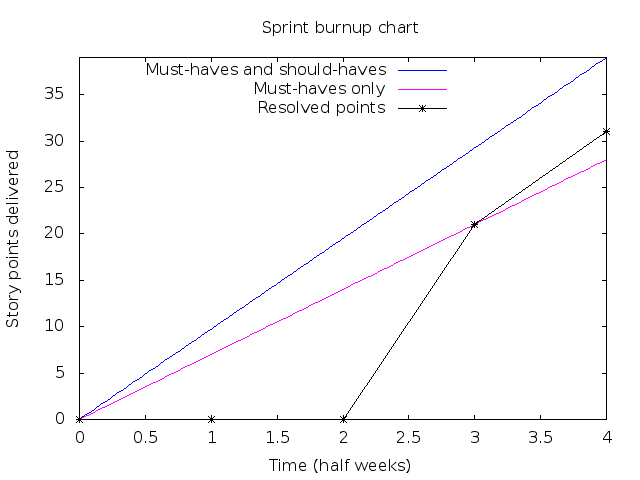
\includegraphics[width=12cm]{img/burnup.png}
	\caption{A burnup graph of our sprint 4.}
	\label{fig:burnup}
\end{figure}

As seen from our burnup graph in figure \ref{fig:burnup}, we completed all our
must-have tasks and some of our should-haves, which marks this as the most
successful sprint to date. Although we did not close any tickets
in the first week, this time was not wasted, but instead spent preparing for
when Jenkins officials granted us publishing right. This also explains the surge
of completed tasks after this quiet-period.

This sprint emphasized what we learned in the previous sprints: While being more
in line with the Scrum principles, shorter sprints yields better results for our
group due to frequent customer meetings and constantly looming deadlines.

\section{Sprint learning goal}
\label{sec:learning_goals}
For this sprint we were asked to analyse and model our development process in
order to improve our process for the coming sprint.

During the previous sprint we have run into several issues, ranging from major
bottlenecks to minor inconveniences, related to our Scrum approach. Most important
of these are the bottlenecks introduced during the Scrum task identification and
description. These tasks often exhibit strong inter-dependence, making it hard to
work on a task without having to wait for someone else. This resulted in unnecessary
downtime which of course is undesirable. 

Furthermore, during the previous sprints, we have experienced how meetings tend
to drag out when done in front of our computers. For this reason we tried to
use stand-up-meetings during this sprint, forcing us away from distractions of
the screen as well as encouraging us to resolve the meeting quickly.

Lastly, we have been notoriously bad at documenting the actual amount of time
spent on each task. Even though we have slowly evolved an unspoken agreement of
how much a story point is, the lack of concrete numbers make this hard to
verify and fine-tune. However, as we are working in story points instead of 
man-hours, we have no way of quantifying the amount of story points spent on a
given task, making this improvement infeasible. 

Having looked into Kanban, we decided against using it for our upcoming sprint
due to the following three reasons. Firstly, since many of our tasks often depend
on each other in a complex manner, we would experience conflicts with the Kanban
work-queue, as we could end in a dead-lock if following the Kanban rules to the
letter. Secondly, we use deadlines as motivation to close outstanding tasks. As
Kanban does not use deadlines in quite the same manner, this process seem unfit
for us. Thirdly, let's not go to Kanban, it has a silly name.

For the coming sprint we have planned our tasks in as non-overlapping a way as
possible. Although we have done this during the entire course, for this sprint
we tried to part the tasks in even smaller tasks to help the problem.

Also, we will continue to use stand-up meetings, as we have found these to help
our productivity greatly.

\section{Coming sprint}
Even though the customer was satisfied with our release, we still have a lot of
work ahead of us. The clone-based approach we have applied to our plugin until
now must be replaced by a branch-based one, as this is more in line with what the
customer is currently doing in other plugins. The reasons we chose a clone-based
approach in the first place, have since vanished.

The customer asked us to further generalize our approach, which means we have to
split our plugin into a generic plugin and a Mercurial specific plugin for our
plugin. This separation of concerns will allow other users to trivially develop
funcitonality for other SCMs than Mercurial, which is a highly desired feature.

This branch-based approach and generalization will be the main focus of the coming
sprint.
\end{document}
